\renewcommand{\rothead}[2][90]{\makebox[0mm][l]{\rotatebox{#1}{\makecell[c]{#2}}}}%
\renewcommand{\arraystretch}{1.4}

\newcommand*\node[1]{
\unitlength1ex
\begin{picture}(2.5,2.5)
\put(0.75,0.75){
	\circle{3}}
	\put(0.7,0.7){
		\makebox(0,0){#1}
	}
\end{picture}
}

\section{Introduction}
Decomposing music into its original audio sources can be a challenging task. Source separation methods can be analyzed how well they perform mathematically, but a human versus machine comparison is cumbersome because measurement of the human separation performance is problematic. One can easily evaluate if humans can detect the number of sources in a mixture of several sources. However, there are indications that even for this task, humans tend to fail if more than three sources are present at the same time \cite{huron89}. Therefore, we want to take a first step by designing an experiment where we focus on polyphonic music of inhomogeneous timbre, where the question is: What is the number of instruments humans can estimate correctly? Several results are addressed in this paper including a possible upper limit of the number of perceived instruments, but also if one can see significant differences in performance of musicians compared to non-musicians. Such results can be used in auditory modeling or as a pre-processing step for source separation algorithms.
This paper presents the results of an experiment, a detailed description of the stimuli and the statistical methods that were used.
\vspace{-1.0em}
\section{Related Work}
The perception of concurrent sound sources has been analyzed on different scales so far. Bregman's and McAdams' \cite{mcadams79} auditory stream theory can be seen as an analytical way of describing how sound events are perceived by the human auditory system. Unfortunately, it is difficult to model professionally produced music by auditory stream models because of its high complexity. As described by Wang \cite{wang2006} there exist several algorithms to estimate the actual number of sources. However, none of them is motivated to model the perceived number of musical sources. Kashino et. al \cite{kashino1995} addresses the questions for concurrent speakers in a ``cocktail party'' like environment and found an upper limit of three voices humans can perceive. When the focus shifts to musical instruments as sources, research has to take concepts from musicology into account. Huron \cite{huron89} was the first who addressed this question in 1989 at a musically meaningful level. Huron asked for the number of voices within a piece of music, where by voices in musicology one can define it as a line of sound or note events (See \cite{cambouropoulos2008voice} for further definitions). Huron determined by experimental results that the number of correctly identified voices is up to three. Later in 1996, Reuter \cite{reuter96} has analyzed how combinations of different instruments are perceived which sets the focus on different instrumentation and not on denumerability.
\vspace{-1.0em}
\section{Experiment}
For the purpose of gaining more knowledge in understanding the human perception of multiple present instruments, an experiment was conducted. Huron selected voices from organ pieces only. We wanted to address the more general case where voices are played by different instruments. Therefore we used a method between musicology and auditory stream analysis to address this question. As we set our focus mainly on comparison between musicians and non-musicians, our experiment was designed so that it respects the fact that the latter have only limited musical background.

Although it might be interesting to have direct comparison with Huron's experiment, we agree that expanding the methods to an inhomogeneous timbre case is error prone. One reason is that there is reasonable doubt about the non-musicians understandings in terms of how a voice is defined. This is why we choose a trade-off with a more simplified experiment where we asked for the number of instruments instead of voices. Also whereas Huron \cite{huron89}  excluded subjects from his experiment because of their lower performance, we compared the results of both groups.
\vspace{-1.0em}
\subsection{Stimuli}

The selection of music items is crucial for our experiment setup. Usually music recordings have no ground truth metadata available to determine the actual number of instruments. Using annotated music like that from the RWC database \cite{rwc} fulfills this requirement but lacks the possibility to remix, attenuate or suppress specific sources. This is important so that the experiment consists of equally grouped stimuli. Instead of the original RWC recordings, the annotated MIDI data itself was used as prototypes for the stimuli.

To make the counting task less ambiguous for the subjects, the instrumentation needs to be mostly constant during the music piece. Therefore we calculated an ``instrumental stationarity'' measure. The annotated MIDI files from \cite{rwc} were converted into piano roll representations for each instrument channel. This representation was then converted into a binary \emph{instrumentation activity matrix} $\mathbf{I}_{AM}\lbrack \mathbf{\underline{k}}_1 \vert \mathbf{\underline{k}}_2 \vert  ... \vert \mathbf{\underline{k}}_N \rbrack \in \{0,1\}$, where at each discrete time instant $i$ a vector $\mathbf{\underline{k}}_i$ indicates which instruments are active. The aim is then to select frames of length $N$ which are stationary by means of changes in instrumentation and activity. To get many items with a high instruments count, the maximum number of instruments within a frame was stored in a binary mask $\mathbf{\underline{k}}_{max}$ which was compared with all $\mathbf{\underline{k}}_{i=1...N}$ so that $(\vert\mathbf{\underline{k}}_{i} \oplus \mathbf{\underline{k}}_{max}\vert \leq 1) \lor (\mathbf{\underline{k}}_{i} = \underline{0})$. The resulting binary vector was smoothed with an averaging kernel of size $N$. By peak picking we got a list of possible candidates which contained a high stationarity in instrumentation.
Further the RWC files were filtered a priori to exclude items dominated by electronic instruments or singing voice. Table~\ref{tab:items} presents the selected 12 items representing pairs of one to six simultaneously present instruments. Each item is around seven seconds long. By cutting at note offsets we varied the lengths of the items to make it semantically more meaningful. Six items (notated as RM-C***) belong to the classical western music genre whereas the other items are of mixed genre.

The MIDI files were humanized randomly and rendered in a professional sequencer software utilizing state-of-the-art commercial sampling products. The rendered files were processed with convolutive reverb to better match the original recordings. Additionally equalization were applied to take loudness measures according to \textsc{EBU R128} recommendations into account. To avoid spatial cues every item was rendered to mono at 16 bit/44.1 kHz.

\begin{table}[h]
\center
\tiny
\begin{tabular}{c|r@{.}l|r@{.}l|l|l|l|l|l|l|l|l|l|l|l|l|l|l|l|l|l|l}
\toprule[1.5pt]

	\multicolumn{5}{l}{ } &
	\multicolumn{18}{c}{Instrument Name} \\

	RWC-MDB ID
	& \multicolumn{2}{c}{Start [s]}
	& \multicolumn{2}{c|}{Dur. [s]}
	& \rothead{Piano}
	& \rothead{Acoustic Guitar}
	& \rothead{Electric Guitar}
	& \rothead{Contrabass (pizz.)}
	& \rothead{Electric Bass}
	& \rothead{Violin}
	& \rothead{Viola}
	& \rothead{Violoncello}
	& \rothead{Contrabass}
	& \rothead{Trumpet}
	& \rothead{Trombone}
	& \rothead{French Horn}
	& \rothead{Tenor Sax}
	& \rothead{Oboe}
	& \rothead{Bassoon}
	& \rothead{Clarinet}
	& \rothead{Flute}
	& $\sum$ \\
	\midrule \hline
J021** & 46&5	& 6&6 & \cellcolor[gray]{0.9} $\times$& & & \cellcolor[gray]{0.9} $\times$& & & & & & \cellcolor[gray]{0.9} $\times$& & & & & & & & 3\\ \hline  \hline
C001 & 0&0 	& 9&0 & & & & & & & & & & & & & & & \cellcolor[gray]{0.9} $\times$& & & \multirow{2}{*}{1} \\
G047 & 35&3	& 8&3 & & & & & & & & \cellcolor[gray]{0.9} $\times$& & & & & & & & & &  \\ \hline
C016 & 0&9	& 7&6 & & & & & & & \cellcolor[gray]{0.9} $\times$ &\cellcolor[gray]{0.9} $\times$& & & & & & & & & & \multirow{2}{*}{2} \\
G068 & 132&4 & 6&6 & & & & & &\cellcolor[gray]{0.9} $\times$& & & & & & & & & & &\cellcolor[gray]{0.9} $\times$ & \\ \hline
C018 & 240&4	& 5&4 &\cellcolor[gray]{0.9} $\times$& & & & &\cellcolor[gray]{0.9} $\times$& & & & & &\cellcolor[gray]{0.9} $\times$& & & & & & \multirow{2}{*}{3} \\
G046 & 0&3	& 7&9 &\cellcolor[gray]{0.9} $\times$& & & & & & &\cellcolor[gray]{0.9} $\times$&\cellcolor[gray]{0.9} $\times$& & & & & & & & & \\ \hline
C013 & 5&6 	& 6&0 & & & & & &\cellcolor[gray]{0.9} $\times$&\cellcolor[gray]{0.9} $\times$&\cellcolor[gray]{0.9} $\times$& & & & & & & & &\cellcolor[gray]{0.9} $\times$ & \multirow{2}{*}{4} \\
G036 & 0&0	& 6&5 &\cellcolor[gray]{0.9} $\times$&\cellcolor[gray]{0.9} $\times$& & &\cellcolor[gray]{0.9} $\times$&\cellcolor[gray]{0.9} $\times$& & & & & & & & & & & & \\ \hline
C012 & 112&0 & 6&0 & & & & & &\cellcolor[gray]{0.9} $\times$&\cellcolor[gray]{0.9} $\times$&\cellcolor[gray]{0.9} $\times$&\cellcolor[gray]{0.9} $\times$& & & & & & & &\cellcolor[gray]{0.9} $\times$ & \multirow{2}{*}{5} \\
G037 & 67&1	& 7&0 &\cellcolor[gray]{0.9} $\times$&\cellcolor[gray]{0.9} $\times$& &\cellcolor[gray]{0.9} $\times$& & & & & & & & &\cellcolor[gray]{0.9} $\times$& & & &$\cellcolor[gray]{0.9} \times$ & \\ \hline
C001 & 147&8 & 6&0 & & & & & &\cellcolor[gray]{0.9} $\times$& & &\cellcolor[gray]{0.9} $\times$& & &\cellcolor[gray]{0.9} $\times$& &\cellcolor[gray]{0.9} $\times$&\cellcolor[gray]{0.9} $\times$&\cellcolor[gray]{0.9} $\times$& & \multirow{2}{*}{6} \\
G028 & 17&5 	& 6&5 &\cellcolor[gray]{0.9} $\times$& &\cellcolor[gray]{0.9} $\times$& &\cellcolor[gray]{0.9} $\times$& & & & &\cellcolor[gray]{0.9} $\times$&\cellcolor[gray]{0.9} $\times$& & & & & &\cellcolor[gray]{0.9} $\times$ & \\ \hline
\bottomrule[1.5pt]

\end{tabular}
\caption{Selected items from the RWC Music Database \cite{rwc}. Item \emph{J021**} is used as training item.}
\label{tab:items}
\end{table}

\subsection{Methods and Participants}

The experiment was attended by 62 participants, where half of them regularly play a musical instrument. They were asked to count how many different instruments they can hear. 12 items from the test set (Table~\ref{tab:items}) were played back in random order. The experiment was presented by a user interface depicted in Figure~\ref{fig:experiment_ui}. Except for the training item, every subject could play back each stimulus up to three times. Additionally they were asked to estimate how certain they were in their decision (ranged from \emph{uncertain} to \emph{very certain}).
\begin{figure}[h]
	\centering
		\fbox{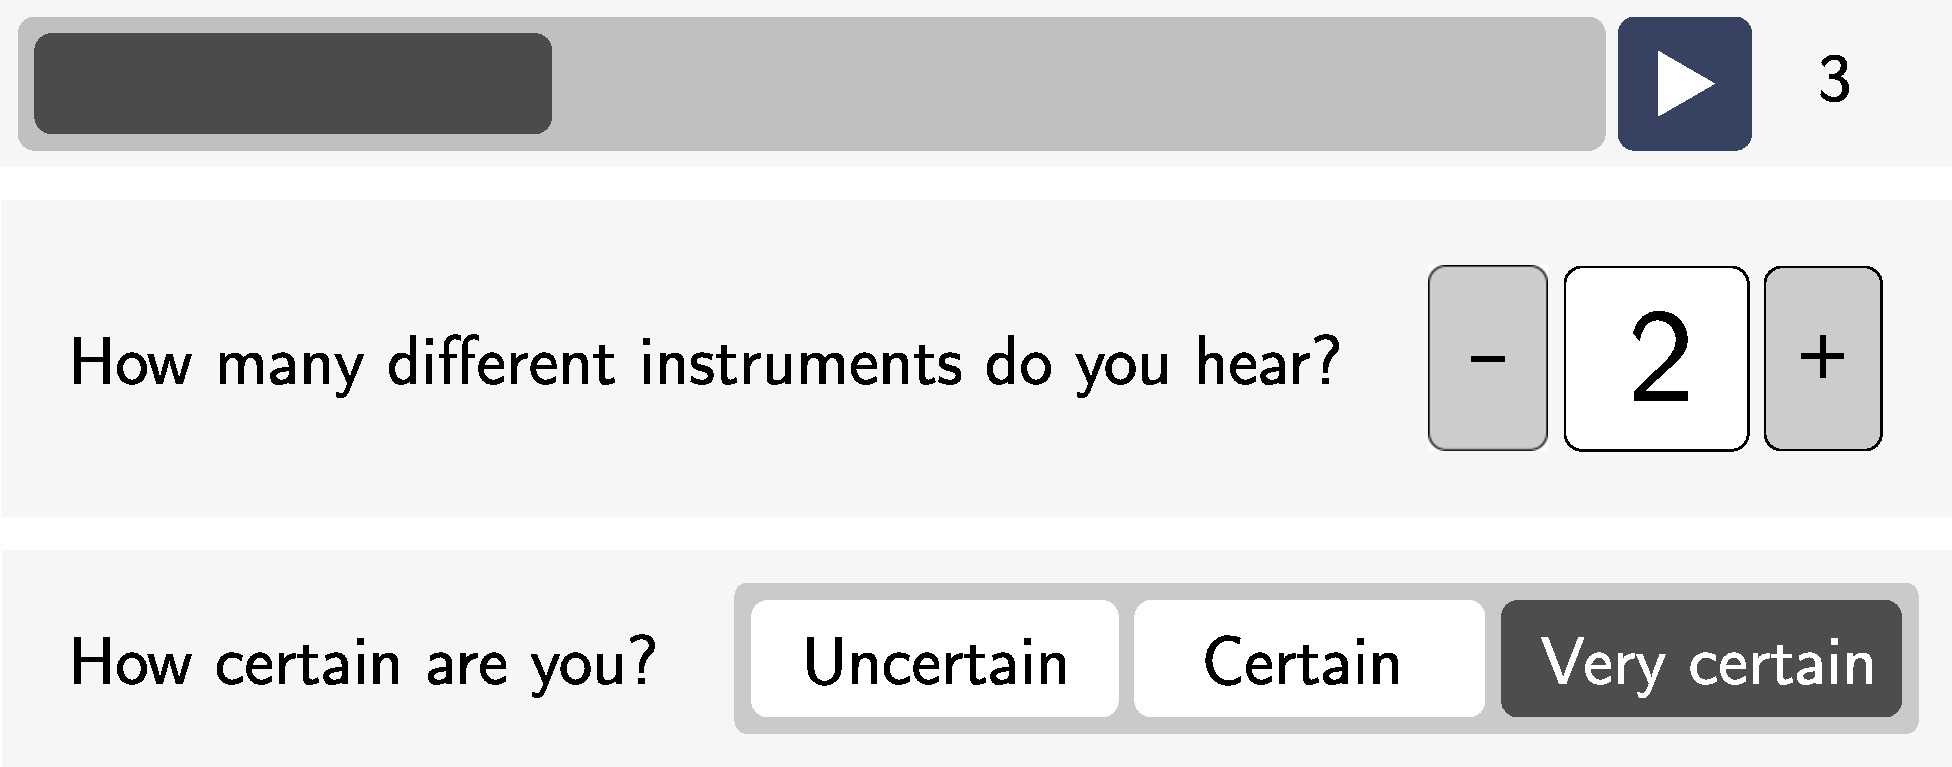
\includegraphics[width=3in]{Chapters/07_Analysis_Experiment/ica/images/userinterface.pdf}}
	\caption{Experiment User Interface}
	\label{fig:experiment_ui}
\end{figure}
Instead of a slider UI-element, the interface only features plus and minus buttons so that the subjects were not biased about the maximum number of instruments. Item \emph{J021**} had been selected as training item and was presented to the subjects during the introduction phase to make them familiar with the user interface. This trial also unveiled the number and name of the instruments within that piece. After they had read the introduction page, the subjects were asked to adjust the volume during the training example to their preference and leave the volume at that level for the duration of the experiment. The stimuli were presented on \textsc{Beyerdynamics DT770} headphones connected to a \textsc{RME Babyface}. The complete test took about 20 minutes on average for every participant.
\vspace{-1.0em}
\section{Results}

The independent variable $I(i)$ is the number of instruments of one music item $i$ where in this case $I(i) \in \{1,2,...,6\}$. $R(i,s)$ is defined as the number of instruments that are perceived and counted by subject $s$ for music item $i$. The dependent variable is the derived from the main subject response as $\Delta(i,s) = I(i) - R(i,s)$ and can also be transformed into a binary scale:
\begin{align*}
	E(i,s)&=\begin{cases}
		0 & \text{if $|\Delta| = 0 $ } \\
		1 & \text{if $|\Delta| > 0 $ .}\\
	\end{cases}
\end{align*}

As we want to address a possible upper bound for the number of instruments that humans are able to correctly count. The primary statistical null hypothesis ($H_1$) is stated in that the means of $\Delta$ and $E$\footnote{The fact that $E$ is dichotomous will lead to a mean value that equals to a probability of a binary distribution.}, grouped by the number of instruments, do not differ significantly. As we also want to test the between-groups performance of musicians versus non-musicians, we introduce another dependent variable $M(s) \in \{0,1\}$ of binary scale. This is stated in a secondary null hypothesis ($H_2$) where the means of $\Delta$ and $E$ are not significantly different between musicians and non-musicians.

The outcome of the experiment is shown in Table~\ref{tab:resultsoverall}. No subjects were screened from the results, although there are two cases where no valid response had been made. Results are grouped by items of $I$ instruments.

In general participants tended to perform worse for items with more than two instruments. The probability of correctly counting one instrument was 90.0\% whereas only one person out of 62 gave a correct response for an item with six instruments. In some cases the number of instruments does not correspond to the number of voices for every item. Items where an instrument plays more than one voice and voices which are played by more than one instrument. However most of the chosen instruments are monophonic so in our case this occured only for items where piano or guitar is present. Also we made sure that the number of total voices did not exceed the maximum number of instruments in that item. Voices being played by more than one instrument are called unisono, which is present in G068, that showed surprisingly good results.
The overall results of the means of $\Delta$ and $E$ are plotted in Figure~\ref{fig:meanerror}.
%!TEX root = ../ica_nautlib.tex
\begin{table}
\begin{center}
\tiny
\begin{tabular}{rrrrrrrrrrrrrrr}
\toprule[1.5pt]
\multicolumn{ 2}{c}{Responses} & \multicolumn{ 13}{c}{Stimuli of RWC-MDB items sorted by number of instruments} \\ 
 \cmidrule(r){1-2} \cmidrule(l){3-15}
 &  & \multicolumn{2}{c}{$I=1$} 
	& \multicolumn{2}{c}{$I=2$} 
	& \multicolumn{2}{c}{$I=3$} 
	& \multicolumn{2}{c}{$I=4$} 
	& \multicolumn{2}{c}{$I=5$} 
	& \multicolumn{2}{c}{$I=6$} 
	& \multicolumn{1}{l}{} \\ 
\cmidrule(r){3-4} \cmidrule(lr){5-6} \cmidrule(lr){7-8} \cmidrule(lr){9-10} \cmidrule(lr){11-12} \cmidrule(l){13-14}
Count & Subject Group &  C001-1 & G047 & C016 & G068 & C018 & G046 & C013 & G036 & C012 & G037 & C001-2 & G028 & n \\ 
\midrule

\multirow{2}{*}{$R=0$} & $M=0$ & 0 & 0 & 0 & 0 & 0 & 0 & 1 & 0 & 0 & 0 & 0 & 0 & 1 \\ 
 & $M=1$ & 0 & 1 & 0 & 0 & 0 & 0 & 0 & 0 & 0 & 0 & 0 & 0 & 1 \\ 
% & $\sum$ & \multicolumn{2}{r}{1} & \multicolumn{2}{r}{0} & \multicolumn{2}{r}{0} & \multicolumn{ 2}{r}{1} & \multicolumn{2}{r}{0} & \multicolumn{2}{r}{0} & 2 \\  

\midrule
\multirow{2}{*}{$R=1$} & $M=0$ & \cellcolor[gray]{0.9} 25 & \cellcolor[gray]{0.9} 30 & 7 & 6 & 0 & 0 & 1 & 1 & 2 & 0 & 1 & 0 & 73 \\ 
 & $M=1$ & \cellcolor[gray]{0.9} 26 & \cellcolor[gray]{0.9} 30 & 7 & 1 & 0 & 0 & 0 & 0 & 0 & 0 & 0 & 0 & 64 \\ 
% & $\sum$ & \multicolumn{2}{r}{\cellcolor[gray]{0.9} 111} & \multicolumn{2}{r}{21} & \multicolumn{2}{r}{0} & \multicolumn{ 2}{r}{2} & \multicolumn{ 2}{r}{2} & \multicolumn{2}{r}{1} & 137 \\  

\midrule
\multirow{2}{*}{$R=2$} & $M=0$ & 6 & 1 & \cellcolor[gray]{0.9} 21 & \cellcolor[gray]{0.9} 25 & 21 & 17 & 14 & 5 & 11 & 7 & 9 & 9 & 146 \\ 
 & $M=1$ & 5 & 0 & \cellcolor[gray]{0.9} 18 & \cellcolor[gray]{0.9} 29 & 6 & 4 & 3 & 3 & 3 & 0 & 3 & 0 & 74 \\ 
% & $\sum$ & \multicolumn{ 2}{r}{12} & \multicolumn{ 2}{r}{\cellcolor[gray]{0.9} 93} & \multicolumn{ 2}{r}{48} & \multicolumn{ 2}{r}{25} & \multicolumn{ 2}{r}{21} & \multicolumn{ 2}{r}{21} & 220 \\  

\midrule
\multirow{2}{*}{$R=3$} & $M=0$ & 0 & 0 & 2 & 0 & \cellcolor[gray]{0.9} 8 & \cellcolor[gray]{0.9} 14 & 11 & 20 & 11 & 17 & 13 & 13 & 109 \\
 & $M=1$ & 0 & 0 & 4 & 1 & \cellcolor[gray]{0.9} 18 & \cellcolor[gray]{0.9} 27 & 19 & 14 & 10 & 11 & 16 & 8 & 128 \\ 
% & $\sum$ & \multicolumn{ 2}{r}{0} & \multicolumn{ 2}{r}{7} & \multicolumn{ 2}{r}{\cellcolor[gray]{0.9} 67} & \multicolumn{ 2}{r}{64} & \multicolumn{ 2}{r}{49} & \multicolumn{2}{r}{50} & 237 \\  

\midrule
\multirow{2}{*}{$R=4$} & $M=0$ & 0 & 0 & 1 & 0 & 2 & 0 & \cellcolor[gray]{0.9} 4 & \cellcolor[gray]{0.9} 4 & 7 & 5 & 6 & 8 & 37 \\
 & $M=1$ & 0 & 0 & 2 & 0 & 7 & 0 & \cellcolor[gray]{0.9} 9 & \cellcolor[gray]{0.9} 13 & 15 & 18 & 5 & 22 & 91 \\ 
% & $\sum$ & \multicolumn{ 2}{r}{0} & \multicolumn{ 2}{r}{3} & \multicolumn{ 2}{r}{9} & \multicolumn{ 2}{r}{\cellcolor[gray]{0.9} 30} & \multicolumn{ 2}{r}{45} & \multicolumn{ 2}{r}{41} & 128 \\  

\midrule
\multirow{2}{*}{$R=5$} & $M=0$ & 0 & 0 & 0 & 0 & 0 & 0 & 0 & 1 & \cellcolor[gray]{0.9} 0 & \cellcolor[gray]{0.9} 2 & 2 & 1 & 6 \\
 & $M=1$ & 0 & 0 & 0 & 0 & 0 & 0 & 0 & 1 & \cellcolor[gray]{0.9} 2 & \cellcolor[gray]{0.9} 2 & 6 & 1 & 12 \\ 
% & $\sum$ & \multicolumn{ 2}{r}{0} & \multicolumn{ 2}{r}{0} & \multicolumn{ 2}{l}{} & \multicolumn{ 2}{r}{2} & \multicolumn{ 2}{r}{\cellcolor[gray]{0.9} 6} & \multicolumn{ 2}{r}{10} & 18 \\  

\midrule
\multirow{2}{*}{$R=6$} & $M=0$ & 0 & 0 & 0 & 0 & 0 & 0 & 0 & 0 & 0 & 0 & \cellcolor[gray]{0.9} 0 & \cellcolor[gray]{0.9} 0 & 0 \\
 & $M=1$ & 0 & 0 & 0 & 0 & 0 & 0 & 0 & 0 & 1 & 0 & \cellcolor[gray]{0.9} 1 & \cellcolor[gray]{0.9} 0 & 2 \\ 
% & $\sum$ & \multicolumn{ 2}{r}{0} & \multicolumn{ 2}{r}{0} & \multicolumn{ 2}{r}{0} & \multicolumn{ 2}{r}{0} & \multicolumn{ 2}{r}{1} & \multicolumn{ 2}{r}{\cellcolor[gray]{0.9} 1} & 2 \\ 
\midrule 
 &  $\sum$& \multicolumn{12}{c}{62 participants, 744 responses} & \\    
\midrule[1pt]
\multirow{3}{*}{Error Probability} & $M=0$ & 0.19 & 0.03 & 0.32 & 0.19 & 0.74 & 0.55 & 0.87 & 0.87 & 1.00 & 0.94 & 1.00 & 1.00 & 0.64 \\ 
 & $M=1$ & 0.16 & 0.03 & 0.42 & 0.06 & 0.42 & 0.13 & 0.71 & 0.58 & 0.94 & 0.94 & 0.97 & 1.00 & 0.53 \\ \cmidrule(r){3-4} \cmidrule(lr){5-6} \cmidrule(lr){7-8} \cmidrule(lr){9-10} \cmidrule(lr){11-12} \cmidrule(lr){13-14} \cmidrule(l){15-15}
 & $\sum$ & \multicolumn{2}{c}{0.10} & \multicolumn{ 2}{c}{0.25} & \multicolumn{2}{c}{0.46} & \multicolumn{2}{c}{0.76} & \multicolumn{ 2}{c}{0.95} & \multicolumn{2}{c}{0.99} & 0.59 \\  
\midrule
\multirow{3}{*}{Mean($\Delta = I-R$)} & $M=0$ & -0.19 & -0.03 & 0.10 & 0.19 & 0.61 & 0.55 & 1.48 & 1.03 & 2.26 & 1.94 & 3.03 & 2.97 & 1.16 \\ 
 & $M=1$ & -0.16 & 0.03 & -0.03 & 0.00 & -0.03 & 0.13 & 0.81 & 0.61 & 1.39 & 1.29 & 2.45 & 2.23 & 0.73 \\ \cmidrule(r){3-4} \cmidrule(lr){5-6} \cmidrule(lr){7-8} \cmidrule(lr){9-10} \cmidrule(lr){11-12} \cmidrule(lr){13-14} \cmidrule(l){15-15}
 & $\sum$ & \multicolumn{2}{c}{-0.09} & \multicolumn{2}{c}{0.06} & \multicolumn{2}{c}{0.31} & \multicolumn{2}{c}{0.98} & \multicolumn{ 2}{c}{1.72} & \multicolumn{2}{c}{2.67} & 0.94 \\ 
\bottomrule[1.5pt]
\end{tabular}
\end{center}
\caption{Experiment results by subjects. Gray background indicates correct responses.}
\label{tab:resultsoverall}
\end{table}


\begin{figure}[h]
\begin{minipage}{0.5\textwidth}
\begin{tabular}{c}
	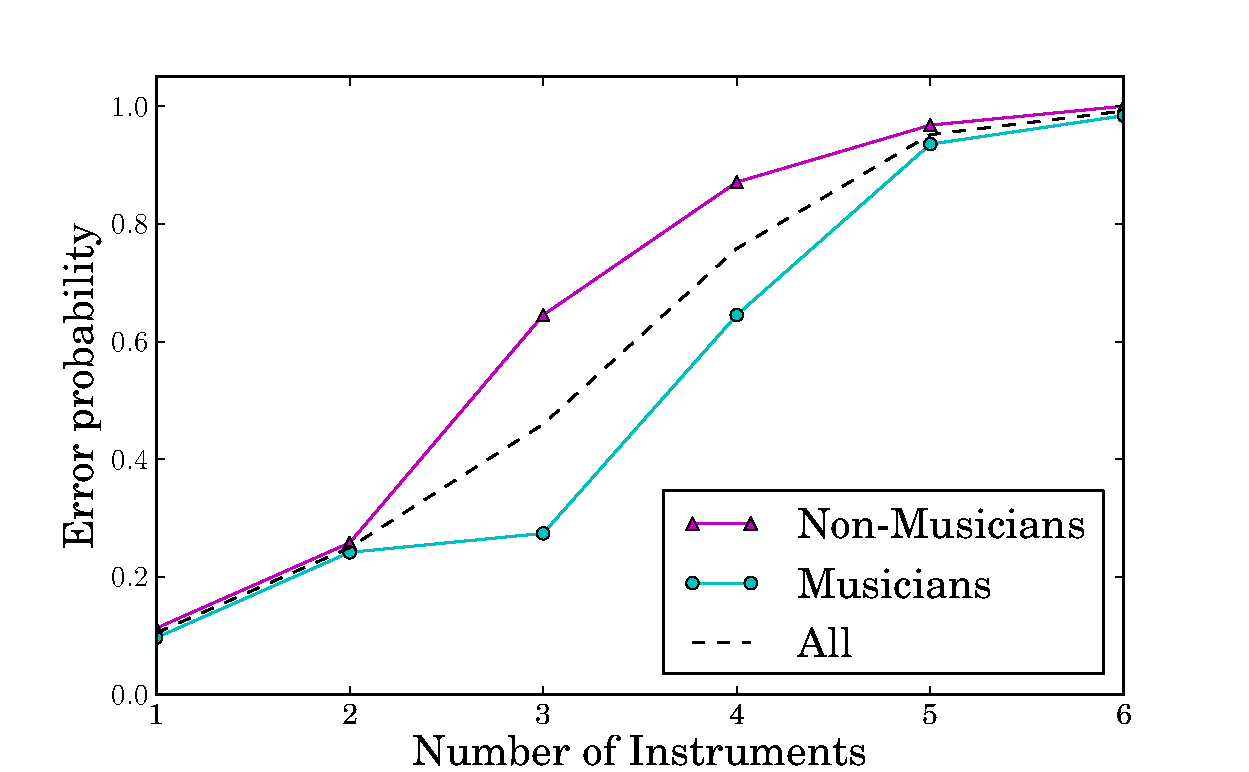
\includegraphics[width=\textwidth]{Chapters/07_Analysis_Experiment/ica/images/error_means.pdf}
\end{tabular}
\end{minipage}
%\hfill
\begin{minipage}{0.5\textwidth}
\begin{tabular}{c}
	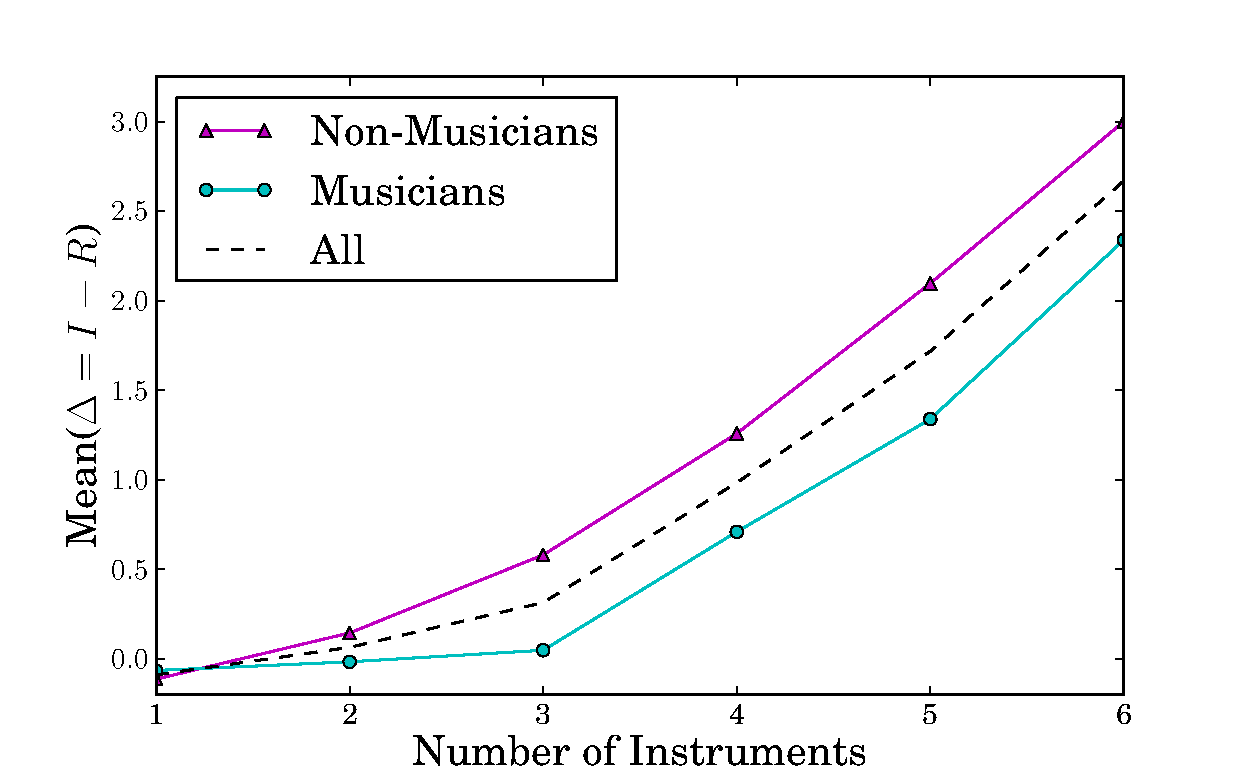
\includegraphics[width=\textwidth]{Chapters/07_Analysis_Experiment/ica/images/error_diff.pdf}
\end{tabular}
\end{minipage}
\caption{Error probability (left) and Mean of $\Delta = I-R$ (right) categorized by the number of instruments.}
\label{fig:meanerror}
\end{figure}
\vspace{-1.0em}

\subsection{Underestimation}

We confirm \cite{huron89} that the most common error is the underestimation of one instrument, although this accounts only for 43 \% of the responses in our experiment. Only in one case $\Delta$ is negative (overestimation) which is item C016, a ``Clarinet Quintet in A major by Wolfgang Amadeus Mozart (K.581. 1st mvmt)'' where we have excluded the solo clarinet part and two strings. Still, the remaining sound seems to be so similar to that of a quartet that musicians tended to hear ``phantom'' instruments.
\vspace{-1.0em}

\subsection{Self-Evaluation}

Figure~\ref{fig:certainty} shows the results of the subjects certainty grouped by instrument count. Although the rate of ``very certain'' responses drops down to 11.3\% for items with six instruments the rate of ``certain'' responses is still as high as 43.5\%. When we take $\Delta$ into account we find a significant linear correlation between $\Delta$ and certainty where 0 is uncertain and 2 is very certain (Pearson's $r = -0.227$ at the $p=0.05$ level).

\begin{figure}[h]
	\centering
		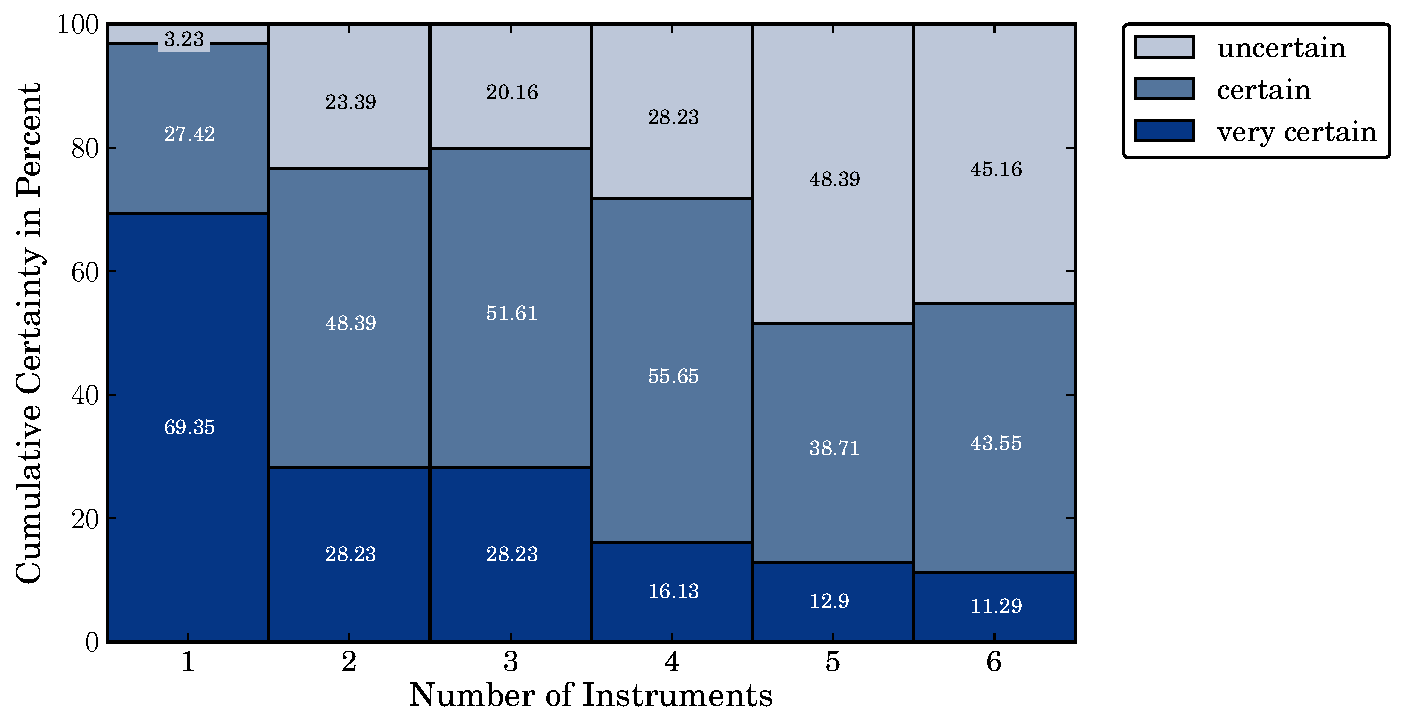
\includegraphics[height=2.5in]{Chapters/07_Analysis_Experiment/ica/images/certainty.pdf}
	\caption{Responses for certainty of subjects by number of instruments}
	\label{fig:certainty}
\end{figure}

\subsection{Main Effects}

Rejecting the null hypotheses ($H_1$ and $H_2$) requires further statistical methods. One reason is that the dependent variables $\Delta$ and $E$ have different scales. We will show that both variables qualify to reject our hypotheses.
As $E$ is dichotomous we focus on $\Delta$ first which can be classified as an interval scaled variable. To show differences between means of two or more groups, usually One-Way-ANOVA tests are applied. ANOVA tests expect independent normally distributed variables and homogeneity of the variances in each group. However both the Kolmogorov--Smirnov test of normal distribution and Levene's test to determine the homogeneity of group variances fail. In such cases variables scaled like $\Delta$ could be transformed so that the boundaries are straightened out. A typically used $arcsin(\sqrt{\Delta})$ transformation was applied to $\Delta$ resulting in slightly higher $p$ values but still not statistically significant. Although ANOVA is known to be robust enough to run the tests against non-normal distributed cases and unequal variances, the significance levels of the results are doubtful. Therefore we choose to run a non-parametric test. The Kruskal--Wallis test can be applied even if the data is not normally distributed. However it has to be run on a slightly modified hypothesis which compares the medians of groups instead of the means. The Kruskal--Wallis test allows to reject both modified hypotheses (asymptotic $p = 0.000$, $\chi^2 = 499636$, $df=5$). As mentioned by \cite{fagerland2009} it may be crucial for the Kruskal--Wallis test to be run on groups with differently shaped distributions. This may not be assured in the case of $\Delta$ as the skewness highly increases for $I \geq 3$. Although the significance of the test has to be treated with caution, the median is a good indicator of a possible upper limit. The overall medians for all groups are plotted in Figure~\ref{fig:median} where one can see that three instruments are a possible upper bound.

\begin{figure}[h]
	\centering
	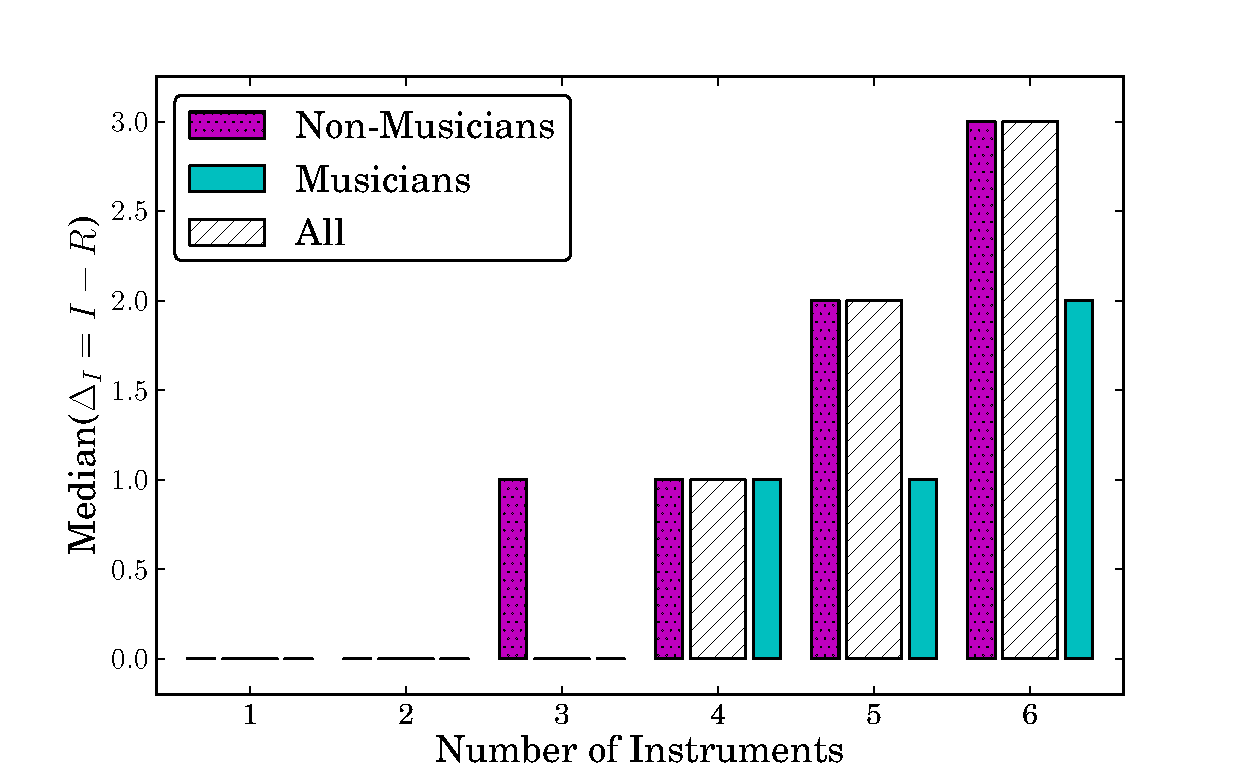
\includegraphics[width=0.6\textwidth]{Chapters/07_Analysis_Experiment/ica/images/diff_medians.pdf}
\caption{Median of $\Delta$ categorized by the number of instruments}
\label{fig:median}
\end{figure}

The reason why an ANOVA is not recommended to be run on $E$ is because it is a categorical variable. Like described in \cite{jaeger2008} this leads to problems which can be avoided by using a binary regression model that turns the mean of $E$ into a an binomial distributed probability. Whereas in standard linear models like ANOVA the output variable will be modeled by a linear equation, in a so called \emph{binary logit regression} the output will be modeled by \emph{log linear} values. By including the main factors $I$ and $M$ we set up a \emph{Generalized Linear Model} (GLM)
\begin{equation}
	logit(E) =  \text{Intercept} + x_1 \text{I} + x_2 \text{M} .
	\label{eq:logit_main}
\end{equation}
A test of the main effects is statistically significant ($\chi^2$ = $437418$, $p < 0.000$, $df = 6$) so that both null hypotheses ($H_1$ and $H_2$) can be rejected. The significance of both effects is shown in Table~\ref{tab:glm_logit} whereas parameter estimates and Wald values of the calculated model are shown in Table~\ref{tab:glm_logit_parameter_estimates}. The intercept represents a constant calculated offset within the regression.

\begin{table}
\center
\scriptsize
\begin{tabular}{cccccc}
\toprule[1.5pt]
Parameter & B & Std. Error & Wald $\chi^2$ & df & Sig. \\
\midrule
(Intercept) & -4.456 & 1.0067 & 19.590 & 1 & .000\\
$M=0$ & -.910 & .2147 & 17.977 & 1 & .000\\
$M=1$ & 0 & . & . & . &  \\
$I=1$ & 7.136 & 1.0507 & 46.131 & 1 & .000\\
$I=2$ & 6.061 & 1.0291 & 34.691 & 1 & .000\\
$I=3$ & 5.081 & 1.0228 & 24.677 & 1 & .000\\
$I=4$ & 3.715 & 1.0274 & 13.076 & 1 & .000\\
$I=5$ & 1.841 & 1.0892 & 2.856 & 1 & .091\\
$I=6$ & 0 & . & . & . & .\\
\bottomrule[1.5pt]
\end{tabular}
\caption{Parameter Estimates for GLM model. Missing values are represented by the Intercept.}
\label{tab:glm_logit_parameter_estimates}
\end{table}

The tests we introduced in the last section show that there is a significant difference in the error probability for groups of different instrumentation but also for musicians versus non-musicians. A pairwise comparison test based on the mean differences reveals where these differences are located. Regarding the error probability of different instrument counts, the pairwise comparison test reveals that nearly all groups show significant mean differences between each other, which was the expected result. However, by calculation using the logit GLM model shown in equation~\ref{eq:logit_main} we found that there are two groups of items of five and six instruments (mean difference $0.04$, std. error = $0.019$, $df = 1$, $p = 0.055$) that did not show any significant difference. For both groups the error probability is close to 100\%.
\subsection{A gap of one instrument between musicians and non-musicians}
To investigate the difference in performance between musicians and non-musicians a pairwise comparison between those two groups was run. Overall musicians perform about 20\% better throughout the test (mean difference = $0.18$, std. error = $ 0.0044$, $df = 1$, $p=0.000$). We do not know what caused these differences as the level of professionalism had not been surveyed. Also 37 \% of the musicians additionally had experience in audio engineering due to their profession. Further to look at possible interaction effects between the number of instruments and the groups of musicians and non-musicians we adapted our logit equation to
\begin{equation}
	logit(E) =  \text{Intercept} + x_1 \text{I} + x_2 \text{M} + x_3 \text{M}\times\text{I} .
	\label{eq:logit_interactions}
\end{equation}
We then reran the GLM analysis selecting only items of three and four instruments. This avoids quasi-complete separation in the logit regression model which is caused by low variances in the error probability for items of $I \in \{1,2,5,6\}$. The model effects of the subset of items are shown in Table~\ref{tab:glm_logit_34}.
\begin{table}
\center
\scriptsize
\begin{minipage}[b]{0.45\textwidth}\centering
	\begin{tabular}{rccc}
	\toprule[1.5pt]
	Source    & Wald $\chi^2$ & df & p \\
	\midrule
	Intercept & 22.643 & 1 & 0.000 \\
	I & 185.359	& 5 & 0.000 \\
	M & 17.977 & 1 & 0.000 \\
	& & & \\
	\bottomrule[1.5pt]
	\end{tabular}
	\caption{Tests of Model Effects of dependent variable $E$ }
    \label{tab:glm_logit}
\end{minipage}
\hfill
\begin{minipage}[b]{0.45\textwidth}
	\begin{tabular}{rccc}
	\toprule[1.5pt]
	Source    & Wald $\chi^2$ & df & p \\
	\midrule
	Intercept & 12.434 & 1 & 0.000 \\
	I & 22.742	& 1 & 0.000 \\
	M & 22.742 & 1 & 0.000 \\
	M$\times$I	& 0.184 & 1 & 0.668 \\
	\bottomrule[1.5pt]
	\end{tabular}
	\caption{Tests of Model Effects of dependent variable $E$ for a subset of items with $I \in \{3,4\}$}
    \label{tab:glm_logit_34}
\end{minipage}
\end{table}

\begin{figure}[h]
	\centering
	\scriptsize
	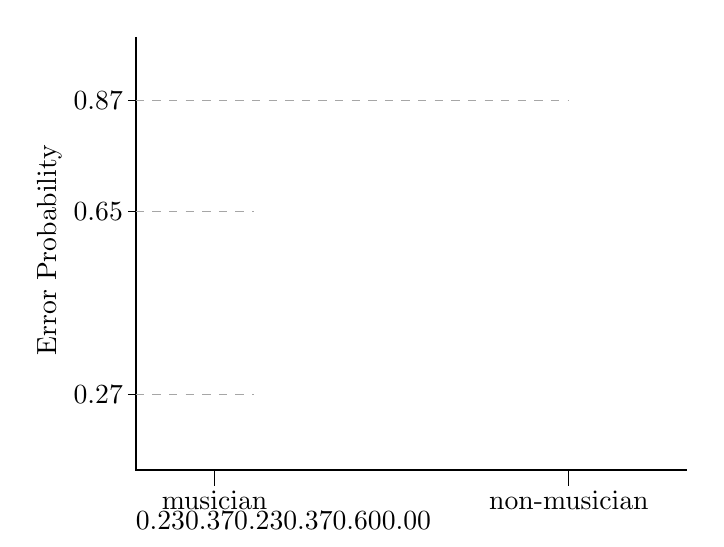
\begin{tikzpicture}[node distance=2cm]
		\draw [-,thick] (0,5*1.25) node (yaxis) [left] {$ $}
	        |- (7,0.75) node (xaxis) {$ $};

		\draw (-1.1, 5) node[left,rotate=90] {Error~Probability};

		\draw (1,-0.2+0.75) -- (1,0+0.75) node[below=4pt] {musician};
		\draw (5.5,-0.2+0.75) -- (5.5,0+0.75) node[below=4pt] {non-musician};

	%	\draw (-0.1, 0) -- (0.1, 0) node[left=4pt] {$0\%$};
		\draw (-0.1, 1.3710*1.25) -- (0.1, 1.3710*1.25) node[left=4pt] {$0.27$};
		\draw (-0.1, 3.2258*1.25) -- (0.1, 3.2258*1.25) node[left=4pt] {$0.65$};
		\draw (-0.1, 4.3548*1.25) -- (0.1, 4.3548*1.25) node[left=4pt] {$0.87$};
	%	\draw (-0.1, 5*1.25) -- (0.1, 5*1.25) node[left=4pt] {$100\%$};

		\draw[dashed,style={color=black!35}] (0, 1.3710*1.25) -- (1.5, 1.3710*1.25) node[left=4pt] {};
		\draw[dashed,style={color=black!35}] (0, 3.2258*1.25) -- (1.5, 3.2258*1.25) node[left=4pt] {};
		\draw[dashed,style={color=black!35}] (0, 4.3548*1.25) -- (5.5, 4.3548*1.25) node[left=4pt] {};

		\GraphInit[vstyle=Normal]
		\tikzset{EdgeStyle/.style={}}
		\tikzset{colorstyle/.style={
			shape= circle,
			line width = 1pt,
			draw = black,
			fill = #1!30}
		}

		\Vertex[L=3,x=1,y=1.3710*1.25,style={colorstyle=red,line width = 4pt}] {3M}
		\Vertex[L=4,x=1,y=3.2258*1.25,style={colorstyle=blue,line width = 2pt}] {4M}
		\Vertex[L=3,x=5.5,y= 3.2258*1.25,style={line width = 4pt}] {3N}
		\Vertex[L=4,x=5.5,y=4.3548*1.25,style={colorstyle=green, draw = black!0,line width = 0}] {4N}

		\Edge[label=$0.23$,style={color=black!50}](3N)(4N)
		\Edge[label=$0.37$,style={color=black!50}](3N)(3M)

		\Edge[label=$0.23$,style={color=black!50}](4N)(4M)
		\Edge[label=$0.37$,style={color=black!50}](4M)(3M)
		\Edge[label=$0.60$,style={color=black!50}](3M)(4N)
		\Edge[label=$0.00$,style={color=red, line width = 2pt}](3N)(4M)

		\end{tikzpicture}
		\caption{Pairwise comparison between interaction of Musician/Non-Musician and the number of instruments (labeled in nodes). The costs between nodes indicates the mean differences between groups. The red/bold line indicates that there is no significant difference at the $p=0.005$ level}
		\label{fig:graph}
\end{figure}
The interaction of Musician$\times$Instruments is not significant on a $p=0.05$ level in general and a pairwise comparison test reveals two groups of equal probability. The pairwise comparisons are depicted in Figure~\ref{fig:graph}. The red vertex indicates there is no significant difference in the error probability for the group of musicians in items with four instruments compared to non-musicians in items of three instruments. Therefore a gap in the error probability of one instrument between those two groups becomes apparent.
\section{Conclusion}
This paper shows that counting the number of instruments in a music item is a difficult task for humans. A new experiment with 62 participants was conducted to address the question of how many instruments one can estimate correctly.
In this experiment, the focus was set on stimuli of inhomogeneous timbre and also mixed genre. By comparing musicians to non-musicians, we revealed that there is a significant difference in performance. Particularly this gap is most prominent for items of three and four instruments. Furthermore, for all stimuli (ranging from one to six instruments) we see that musicians performed about 20\% better than non-musicians. The experiment shows an assumed upper limit for items with more than three instruments. Our results are closely related to a previous experiment which focused on voices instead of instruments.
This work can be used as a basis to define target functions for related research in auditory modeling. Future work could address different groups of items to reveal if certain instrumentations or compositions influence the results.

% \bibliographystyle{jasanum}
%\bibliographystyle{jasaauthyear}
